\section{Line tracking sensor}
\begin{figure}[H]
    \centering
    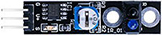
\includegraphics[angle=0, keepaspectratio=true, scale=1, width=200px, height=200px]{images/line_tracking.jpg}
    %\caption{Caption}
\end{figure}
\subsection*{Description}
The line tracking module uses an infrared transmitter and receiver to detect the amount of reflection of the surface in front of it.

The effective distance can range from 2 - 40cm and is adjusted using the potentiometer on the module. A line tracking robot can be implemented using two of these modules (one to check if the robot is drifting left and one to check if the robot is drifting right).

\subsection*{Pin mapping}
This pin mapping corresponds to the pins from left to right with the module pins facing towards you.
\begin{table}[H]
    \centering
    \begin{tabular}{|c|c|c|c|c|}
    \hline
    Index &Label &Type &Name &Description\\ \hline
    0 &G &Ground &GND & \\ \hline
    1 &V+ &Source voltage &$V+$ &Module source voltage ($5V$)\\ \hline
    2 &S &Digital output &D0 &\\ \hline
    \end{tabular}
    %\caption{Caption}
    %\label{tab:my_label}
\end{table}
\subsection*{Operation}
The output voltage at the digital pin (D0) is set to high when the module detects a reflective surface above the set threshold. The circuit is completed when the infrared waves emitted from the transmitter and reflected and absorbed by the infrared receiver.

By adjusting the potentiometer on the module the reflectivity threshold can be changed.
\subsection*{Code}
Refer to listing \ref{python_linetracker}.
%\lstinputlisting[caption=test]{laser.py}